
\documentclass[12pt,a4paper]{article}

\usepackage[english]{babel}
\usepackage[utf8]{inputenc}
\usepackage{amsfonts,amssymb,amsbsy}

\usepackage[ddmmyyyy]{datetime}
\renewcommand{\dateseparator}{.}
\usepackage{amsmath}
\usepackage{gensymb}
\usepackage{subcaption}
\usepackage{array}
\usepackage{graphicx}

%\setlength\abovecaptionskip{-5pt}
\usepackage[margin=1.1in]{geometry}

\usepackage[T1]{fontenc}

\usepackage{hyperref}
\hypersetup{pdfpagemode=UseNone, pdfstartview=FitH,
	colorlinks=true,urlcolor=red,linkcolor=black,citecolor=black}
	
\usepackage{tikz}
\usetikzlibrary{positioning}
	
\usepackage[backend=biber,
style=numeric-comp,
sorting=none,
maxbibnames=8
]{biblatex}
\addbibresource{bib.bib}
\AtEveryBibitem{
 \clearfield{url}
 \clearfield{month}
}

\frenchspacing


\begin{document}
	
	\title{Deep learning for materials and textures.}
	\author{Niko Oinonen}
	\maketitle
	
	\noindent
	The identification of material and textures in images is a challenging task. The same material can have many different appearances in different situations depending on factors such as the more specific type of material (e.g. different types of wood), lighting and weather conditions (e.g. wet surface), and viewing angle. Various methods based on, for example, feature engineering \cite{liu_2010}, auto-encoders \cite{li_2014}, and convolutional neural networks \cite{kalliatakis_2016} have been tried. This work investigates the use of convolutional neural networks in identifying materials and textures in images. Code is available at \url{https://github.com/NikoOinonen/deeplearning-textures}.
	
	\section{Data and methods}
	
%	\begin{table}
%		\centering
%		\caption{Categories of images present in the databases used in the experiments.}
%		\begin{tabular}{l|c|c|c}
%									& MINC-2500	& FMD 	& KTH-TIPS2-b 	\\ \hline
%			Number of images		& 57500		& 1000	& 4752 			\\ \hline
%			Number of categories	& 23 		& 10 	& 11 			\\ \hline
%			Aluminium foil			& 			&		& X				\\ \hline
%			Brick					& X			&		&				\\ \hline
%			Brown bread				& 			&		& X				\\ \hline
%			Carpet					& X			& 		&				\\ \hline
%			Ceramic					& X			&		&				\\ \hline
%			Corduroy				& 			&		& X				\\ \hline
%			Cork					& 			&		& X				\\ \hline
%			Cotton					& 			&		& X				\\ \hline
%			Cracker					& 			&		& X				\\ \hline
%			Fabric					& X			&	X	&				\\ \hline
%			Foliage					& X			&	X	&				\\ \hline
%			Food					& X			&		&				\\ \hline
%			Glass					& X			&	X	&				\\ \hline
%			Hair					& X			&		&				\\ \hline
%			Leather					& X			&	X	&				\\ \hline
%			Lettuce leaf			& 			&		& X				\\ \hline
%			Linen					& 			&		& X				\\ \hline
%			Metal					& X			&	X	&				\\ \hline
%			Mirror					& X			&		&				\\ \hline
%			Other					& X			&		&				\\ \hline
%			Painted					& X			&		&				\\ \hline
%			Paper					& X			&	X	&				\\ \hline
%			Plastic					& X			&	X	&				\\ \hline
%			Polished stone			& X			&		&				\\ \hline
%			Skin					& X			&		&				\\ \hline
%			Sky						& X			&		&				\\ \hline
%			Stone					& X			&	X	&				\\ \hline
%			Tile					& X			&		&				\\ \hline
%			Wallpaper				& X			&		&				\\ \hline
%			Water					& X			&	X	&				\\ \hline
%			White bread				& 			&		& X				\\ \hline
%			Wood					& X			&	X	& X 			\\ \hline
%			Wool					& 			&		& X 			\\ \hline
%		\end{tabular}
%		\label{table:stats}
%	\end{table}

	\begin{table}
		\centering
		\caption{Categories of images present in the databases used in the experiments.}
		\begin{tabular}{l|c|c|c}
									& MINC-2500	& FMD 	\\ \hline
			Number of images		& 57500		& 1000	\\ \hline
			Number of categories	& 23 		& 10 	\\ \hline
			Brick					& X			&		\\ \hline
			Carpet					& X			& 		\\ \hline
			Ceramic					& X			&		\\ \hline
			Fabric					& X			&	X	\\ \hline
			Foliage					& X			&	X	\\ \hline
			Food					& X			&		\\ \hline
			Glass					& X			&	X	\\ \hline
			Hair					& X			&		\\ \hline
			Leather					& X			&	X	\\ \hline
			Metal					& X			&	X	\\ \hline
			Mirror					& X			&		\\ \hline
			Other					& X			&		\\ \hline
			Painted					& X			&		\\ \hline
			Paper					& X			&	X	\\ \hline
			Plastic					& X			&	X	\\ \hline
			Polished stone			& X			&		\\ \hline
			Skin					& X			&		\\ \hline
			Sky						& X			&		\\ \hline
			Stone					& X			&	X	\\ \hline
			Tile					& X			&		\\ \hline
			Wallpaper				& X			&		\\ \hline
			Water					& X			&	X	\\ \hline
			Wood					& X			&	X	\\ \hline
		\end{tabular}
		\label{table:stats}
	\end{table}
	
	The datasets used for experiments here are the Materials in Context Database (MINC) \cite{bell_2015} and the Flickr Material Database (FMD) \cite{sharan_2010}. Here the smaller MINC-2500 version of the MINC database is used. MINC-2500 consists of images in 23 different categories with 2500 images in each category, and FMD has 10 categories with 100 image in each category. Table \ref{table:stats} lists all the categories present in the databases. From the table we can note that the categories in FMD are a subset of the categories in the MINC-2500 database. Both databases are divided into training/validation/test sets in 0.6/0.1/0.3 proportions, respectively.
	
	Figure \ref{fig:examples} shows some example images from the datasets. In addition to size, the biggest difference between the databases is that in FMD the material to be recognized occupies most of the image, whereas in MINC there is more context around the material object, as the name of the database implies.
	
	\begin{figure}
		\centering
		\captionsetup[subfigure]{labelformat=empty}
		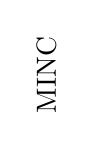
\begin{tikzpicture}
			\node [rotate=90] {MINC};
		\end{tikzpicture}
		\begin{subfigure}[c]{0.23\linewidth}
			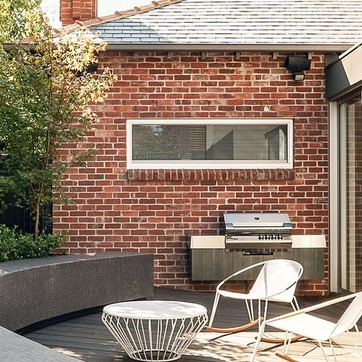
\includegraphics[width=\linewidth]{./imgs/minc1}
			\caption{Brick}
			\vspace{5mm}
		\end{subfigure}
		\begin{subfigure}[c]{0.23\linewidth}
			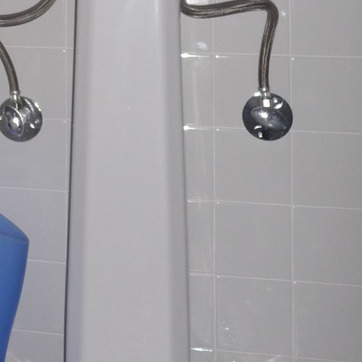
\includegraphics[width=\linewidth]{./imgs/minc2}
			\caption{Ceramic}
			\vspace{5mm}
		\end{subfigure}
		\begin{subfigure}[c]{0.23\linewidth}
			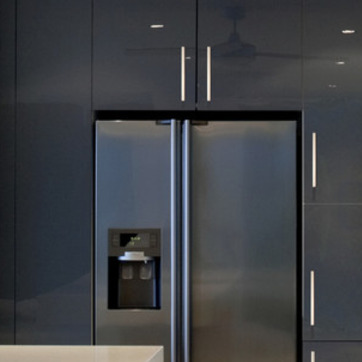
\includegraphics[width=\linewidth]{./imgs/minc3}
			\caption{Metal}
			\vspace{5mm}
		\end{subfigure}
		\begin{subfigure}[c]{0.23\linewidth}
			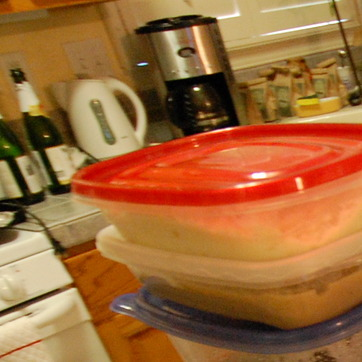
\includegraphics[width=\linewidth]{./imgs/minc4}
			\caption{Plastic}
			\vspace{5mm}
		\end{subfigure}
		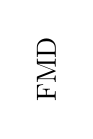
\begin{tikzpicture}
			\node [rotate=90] {FMD};
		\end{tikzpicture}
		\begin{subfigure}[c]{0.23\linewidth}
			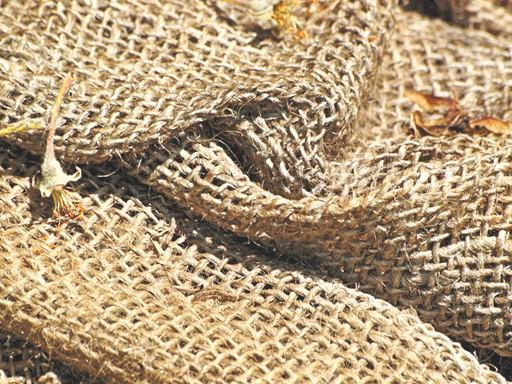
\includegraphics[width=\linewidth]{./imgs/fmd1}
			\caption{Fabric}
			\vspace{2mm}
		\end{subfigure}
		\begin{subfigure}[c]{0.23\linewidth}
			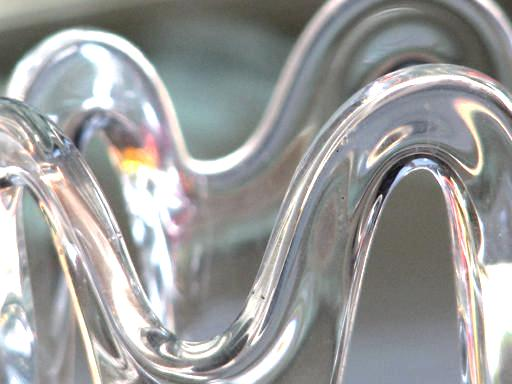
\includegraphics[width=\linewidth]{./imgs/fmd2}
			\caption{Glass}
			\vspace{2mm}
		\end{subfigure}
		\begin{subfigure}[c]{0.23\linewidth}
			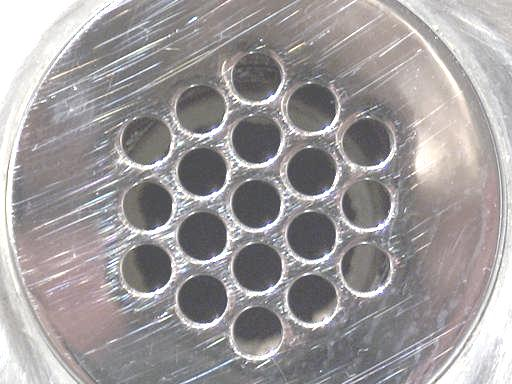
\includegraphics[width=\linewidth]{./imgs/fmd3}
			\caption{Metal}
			\vspace{2mm}
		\end{subfigure}
		\begin{subfigure}[c]{0.23\linewidth}
			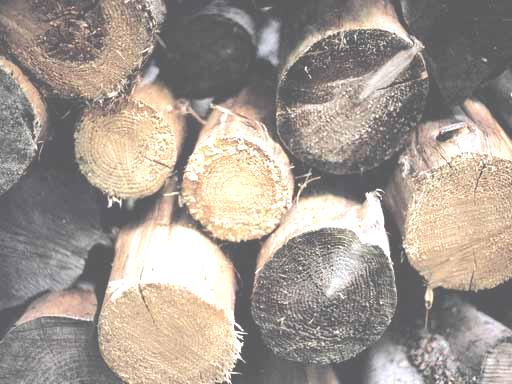
\includegraphics[width=\linewidth]{./imgs/fmd4}
			\caption{Wood}
			\vspace{2mm}
		\end{subfigure}
%		\begin{tikzpicture}
%			\node [rotate=90] {KTH-TIPS2-b};
%		\end{tikzpicture}
%		\begin{subfigure}[c]{0.23\linewidth}
%			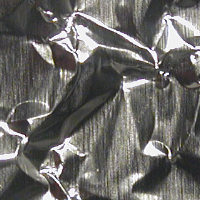
\includegraphics[width=\linewidth]{./imgs/kth1}
%			\caption{Aluminium foil}
%			\vspace{18mm}
%		\end{subfigure}
%		\begin{subfigure}[c]{0.23\linewidth}
%			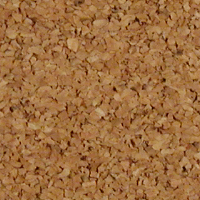
\includegraphics[width=\linewidth]{./imgs/kth2}
%			\caption{Cork}
%			\vspace{18mm}
%		\end{subfigure}
%		\begin{subfigure}[c]{0.23\linewidth}
%			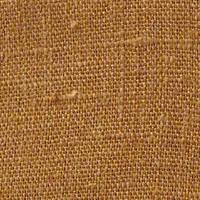
\includegraphics[width=\linewidth]{./imgs/kth3}
%			\caption{Linen}
%			\vspace{18mm}
%		\end{subfigure}
%		\begin{subfigure}[c]{0.23\linewidth}
%			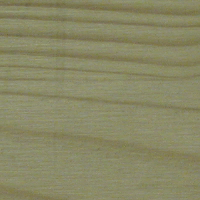
\includegraphics[width=\linewidth]{./imgs/kth4}
%			\caption{Wood}
%			\vspace{18mm}
%		\end{subfigure}
%		\vspace{-18mm}
		\caption{Example images from the datasets.}
		\label{fig:examples}
	\end{figure}
	
	%TODO example images
	
	\subsection{Deep learning models}
	
	\begin{figure}
		\centering
		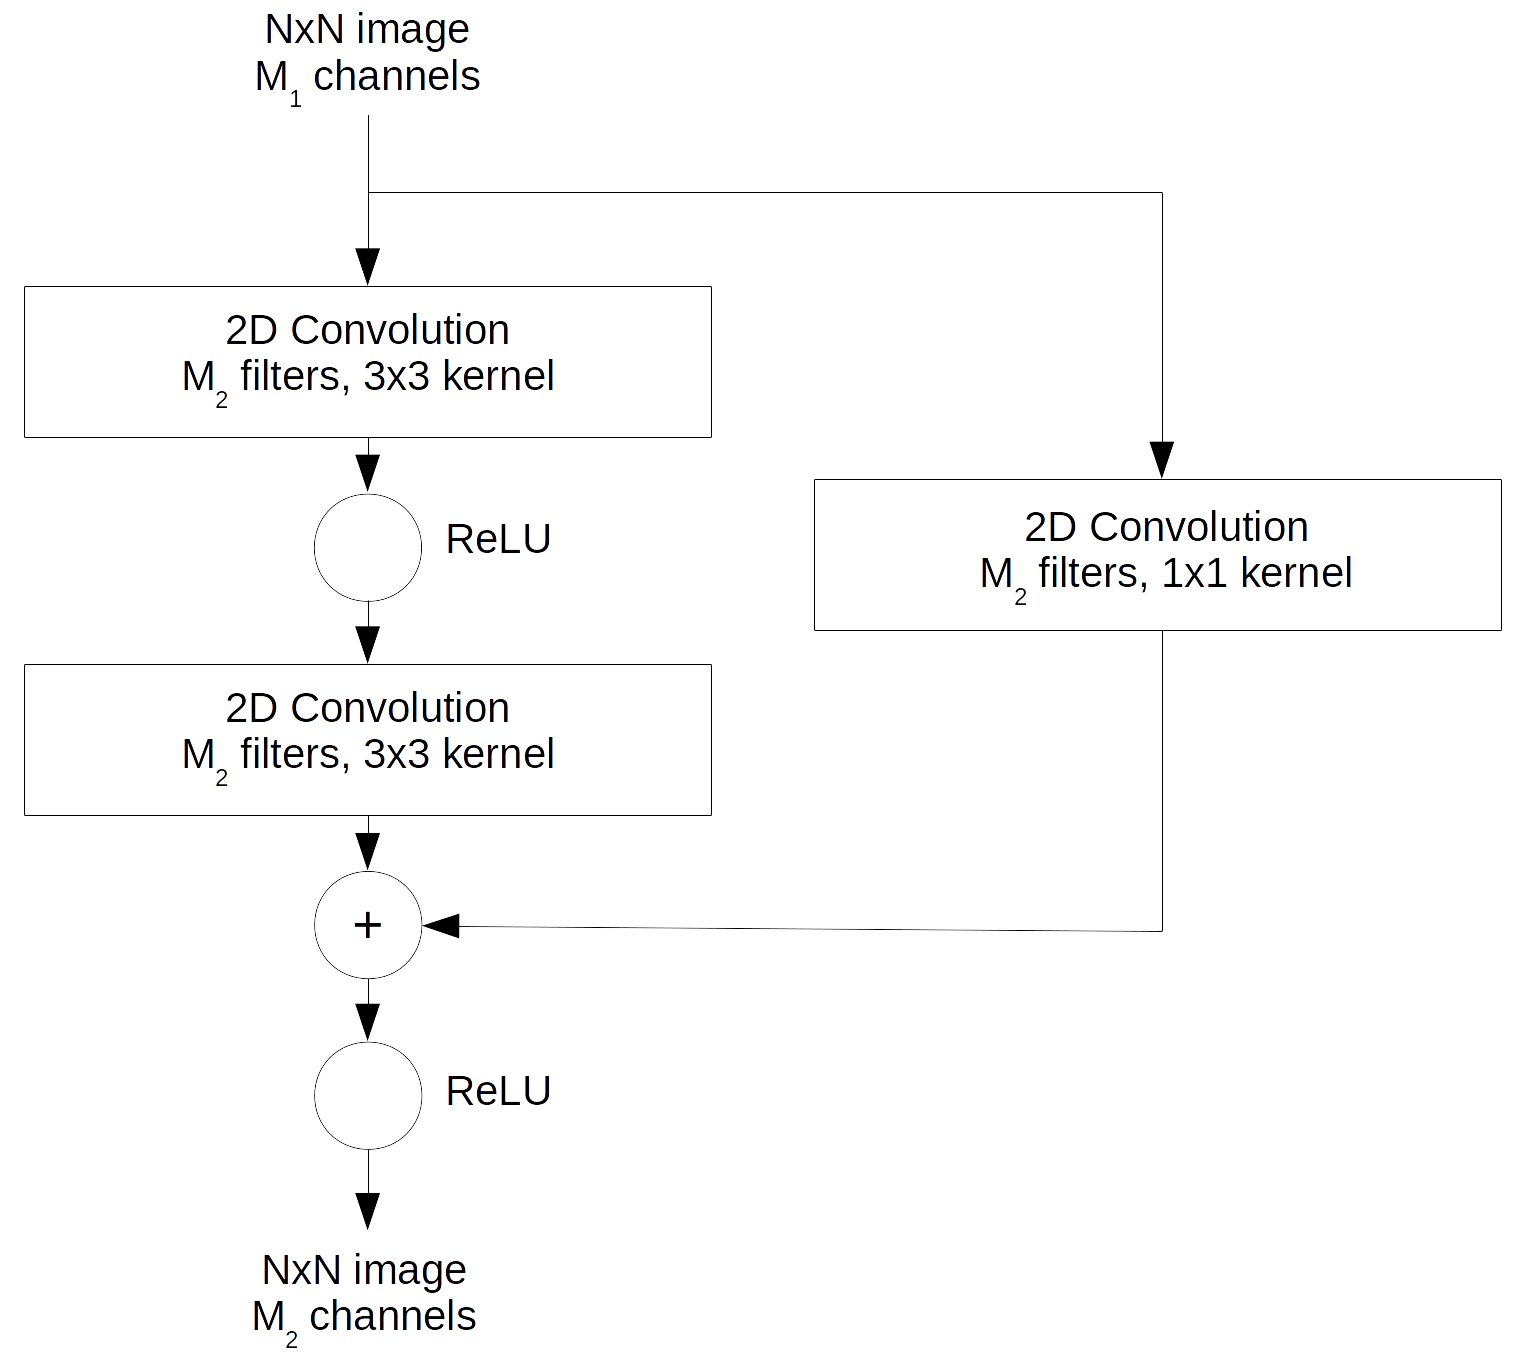
\includegraphics[width=0.7\linewidth]{res_block}
		\caption{Illustration of residual connection block.}
		\label{fig:res_block}
	\end{figure}
	
	\begin{table}[t!]
		\centering
		\caption{Model architecture for MINC-2500 database. Total number of parameters is 152993.}
		\begin{tabular}{l|l l l}
			Layer type  & Dimension & Filters/Pool size/rate & Parameters 	\\ \hline
			Input 		& $128 \times 128 \times 3$  & -  			& -     \\ \hline
			ResBlock 	& $128 \times 128 \times 18$ & 18 			& 3510  \\ \hline
			MaxPool 	& $64 \times 64 \times 18$ & $2 \times 2$	& -     \\ \hline
			ResBlock 	& $64 \times 64 \times 25$ & 25 			& 10200 \\ \hline
			MaxPool 	& $32 \times 32 \times 25$ & $2 \times 2$ 	& -     \\ \hline
			ResBlock 	& $32 \times 32 \times 36$ & 36 			& 20772 \\ \hline
			MaxPool 	& $16 \times 16 \times 36$ & $2 \times 2$ 	& -     \\ \hline
			ResBlock 	& $16 \times 16 \times 72$ & 72 			& 72792 \\ \hline
			AvgPool 	& $3 \times 3 \times 72$   & $5 \times 5$ 	& -	    \\ \hline
			Flatten 	& $648$ 	 			   & -  			& -	    \\ \hline
			Dropout 	& $648$ 	 			   & 0.3  			& -	    \\ \hline
			Dense 		& $68$ 	 			   	   & -  			& 44132 \\ \hline
			Dropout 	& $68$ 	 			   	   & 0.05  			& -	    \\ \hline
			Dense 		& $23$ 	 			   	   & -  			& 1587  \\ \hline
		\end{tabular}
		\label{table:model_minc}
	\end{table}

	\begin{table}[t!]
		\centering
		\caption{Model architecture for FMD database. Total number of parameters is 8554.}
		\begin{tabular}{l|l l l}
			Layer type  & Dimension & Filters/Pool size/rate & Parameters 	\\ \hline
			Input 		& $128 \times 128 \times 3$ & -  			& -     \\ \hline
			ResBlock 	& $128 \times 128 \times 6$ & 6 			& 522   \\ \hline
			MaxPool 	& $32 \times 32 \times 6$   & $4 \times 4$	& -     \\ \hline
			ResBlock 	& $32 \times 32 \times 15$  & 15 			& 2970  \\ \hline
			MaxPool 	& $8 \times 8 \times 15$    & $4 \times 4$ 	& -     \\ \hline
			ResBlock 	& $8 \times 8 \times 12$    & 12 			& 3132  \\ \hline
			MaxPool 	& $4 \times 4 \times 12$    & $2 \times 2$ 	& -     \\ \hline
			Flatten 	& $192$ 	 			    & -  			& -	    \\ \hline
			Dropout 	& $192$ 	 			    & 0.55  		& -	    \\ \hline
			Dense 		& $10$ 	 			   	    & -  			& 1930  \\ \hline
		\end{tabular}
		\label{table:model_fmd}
	\end{table}

	
	
	All the models used here are convolutional neural networks utilizing residual connections (ResNets) \cite{he_2015}. The ResNets are built by stacking residual blocks interleaved by pooling layers and terminating in dense layers for the classification task. See Fig.\ref{fig:res_block} for an illustration of the ResBlock. All the activation functions are ReLUs except the activation of the classification layer, which is Softmax. The models are implemented in Keras \cite{chollet_keras} with Tensorflow \cite{tensorflow} backend.
	
	Due to differences between the databases, a single network cannot be optimal for both of them. In particular, a large number of parameters results in easily overfitting on the smaller FMD database. Tables \ref{table:model_minc} and \ref{table:model_fmd} describe the model architectures used for the different databases. 
	
	The number of filters in different layers and the dropout rates are found with a combination of random and manual search. During random search the training was is when the validation loss has not improved in 10 epochs. The parameters are chosen from the model with the lowest validation loss and the dropout rates are manually adjusted to balance the training and validation loss to be similar. The final model weights are chosen from the epoch with the lowest validation loss. The models weights are optimized with the Adam optimizer \cite{kingma_2014}.
	
	
	\subsection{Data processing and regularization}
	
	The image data is normalized feature-wise by subtracting the mean and dividing by standard deviation. The mean and standard deviation of each feature are computed on the training set. For FMD, the whole training set is used, and for MINC-2500 1000 images from the training set are used. To augment and regularize the training, several random preprocessing steps are used:
	
	\begin{itemize}
		
		\item \textbf{Random flips.} The images are randomly flipped left-to-right with 50\% probability.
		
		\item \textbf{Random crops.}
			The images are cropped to a random location and size between 70\% and 100\% of the original image.
			
		\item \textbf{Random noise.} Uniform random noise with amplitude 0.5 is added to the images after normalization. 
		
	\end{itemize}
	
	\noindent
	The models are additionally regularized by dropouts \cite{srivastava_2014} in the dense layers. The random noise is applied only in the FMD model training. Samples in the validation and test sets are normalized, but no additional preprocessing steps are applied. The images are finally resized to the model input size with nearest-neighbor sampling.
	
	\section{Results}
	
	The trained models reach 58.7\% and 33.3\% accuracies on the test sets of the MINC-2500 and FMD datasets, respectively. Figure \ref{fig:conf} shows the confusion matrices and Table \ref{table:prec_rec} show the precision and recall rates for both of the datasets. If $M_{ij}$ is the confusion matrix element for true class $i$ and predicted class $j$, the precision and recall of a class $i$ are defined as
	\begin{align}
		\mathrm{precision}_i &= \frac{M_{ii}}{\sum_{k=1}^{N_{classes}} M_{ki}}, \\
		\mathrm{recall}_i &= \frac{M_{ii}}{\sum_{k=1}^{N_{\mathrm{classes}}} M_{ik}}.
	\end{align}
	From the confusion matrix and precision and recall rates we can see that most difficult classes for the models are 'Plastic' in MINC-2500 and 'Metal' in FMD. In fact, the FMD model fails to correctly predict any images in the 'Metal' category. The easiest categories are 'Sky' in MINC-2500 and 'Foliage' in FMD.
	
	Figure \ref{fig:losses} shows the training and validation losses during training. On the MINC-2500 dataset the two loss curves are overlapping, meaning that the model is not overfitted on the training data. However, on the FMD dataset the model very quickly overfits to the training set, even with the much smaller model and higher regularization rates.
	
	\begin{figure}
		\centering
		\vspace{-15mm}
		\begin{subfigure}[c]{0.95\linewidth}
			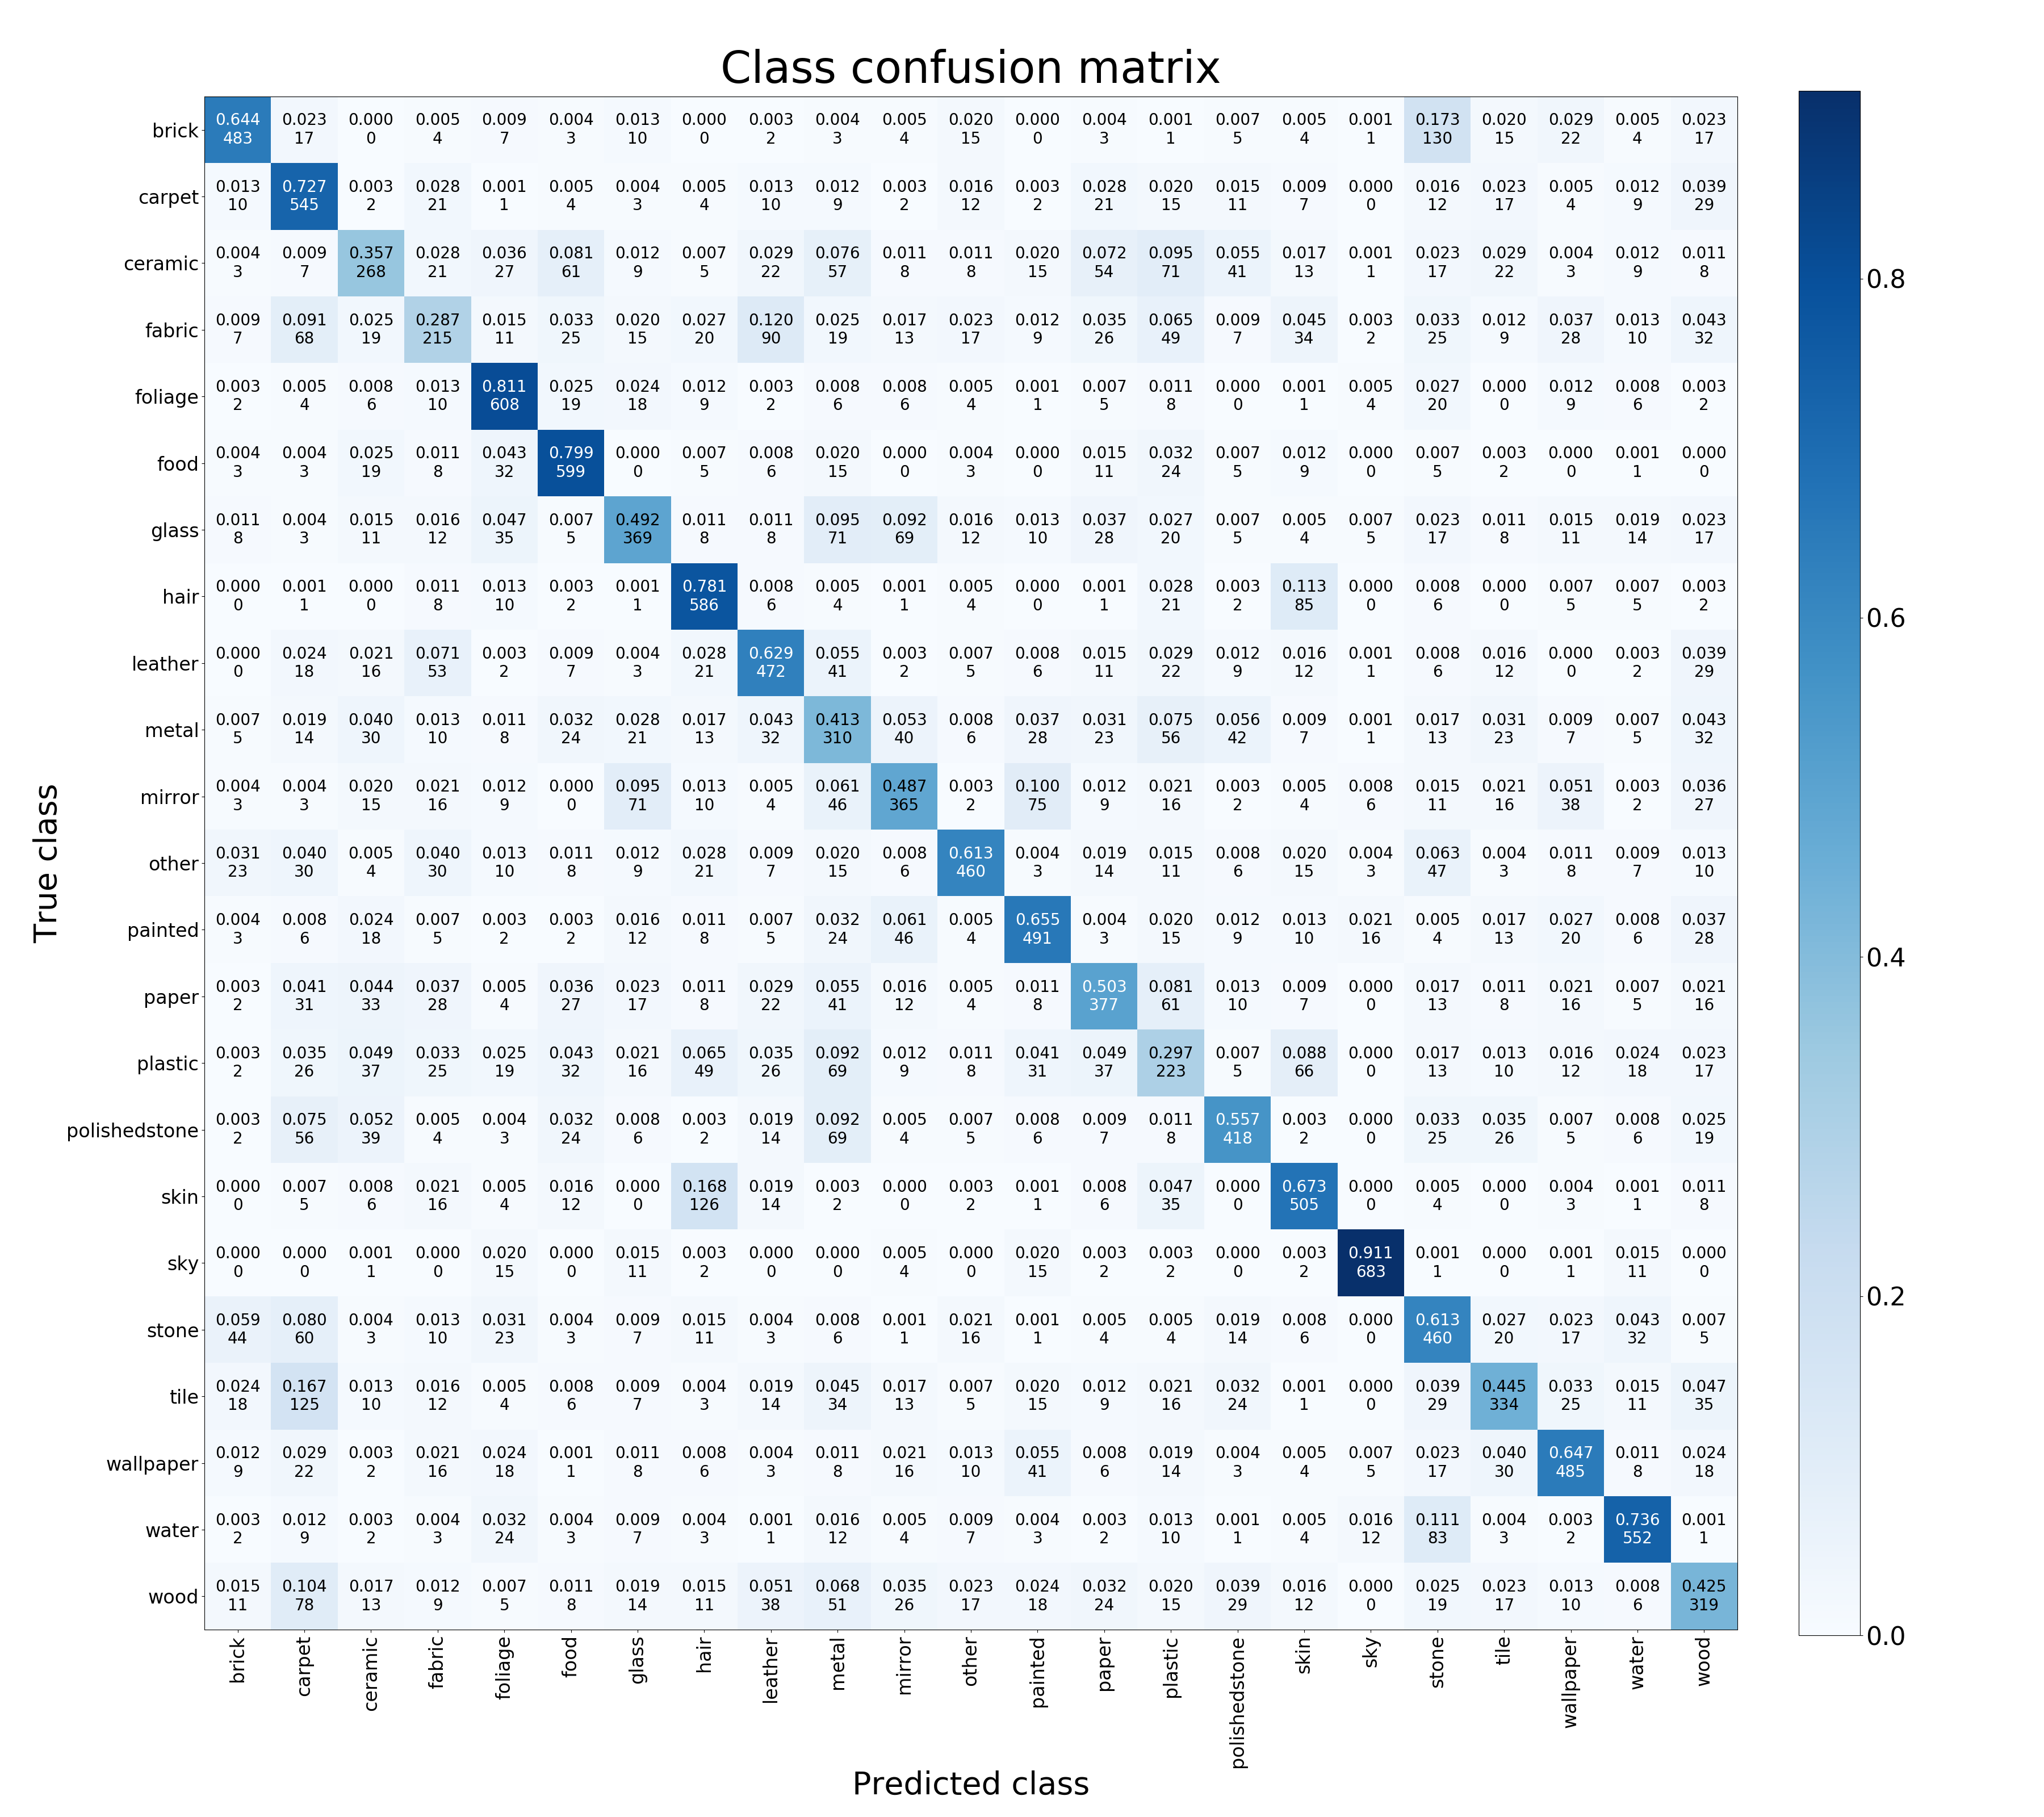
\includegraphics[width=\linewidth]{imgs/conf_minc}
			\caption{}
			\label{fig:confminc}
			\vspace{2mm}
		\end{subfigure}
		\begin{subfigure}[c]{0.7\linewidth}
			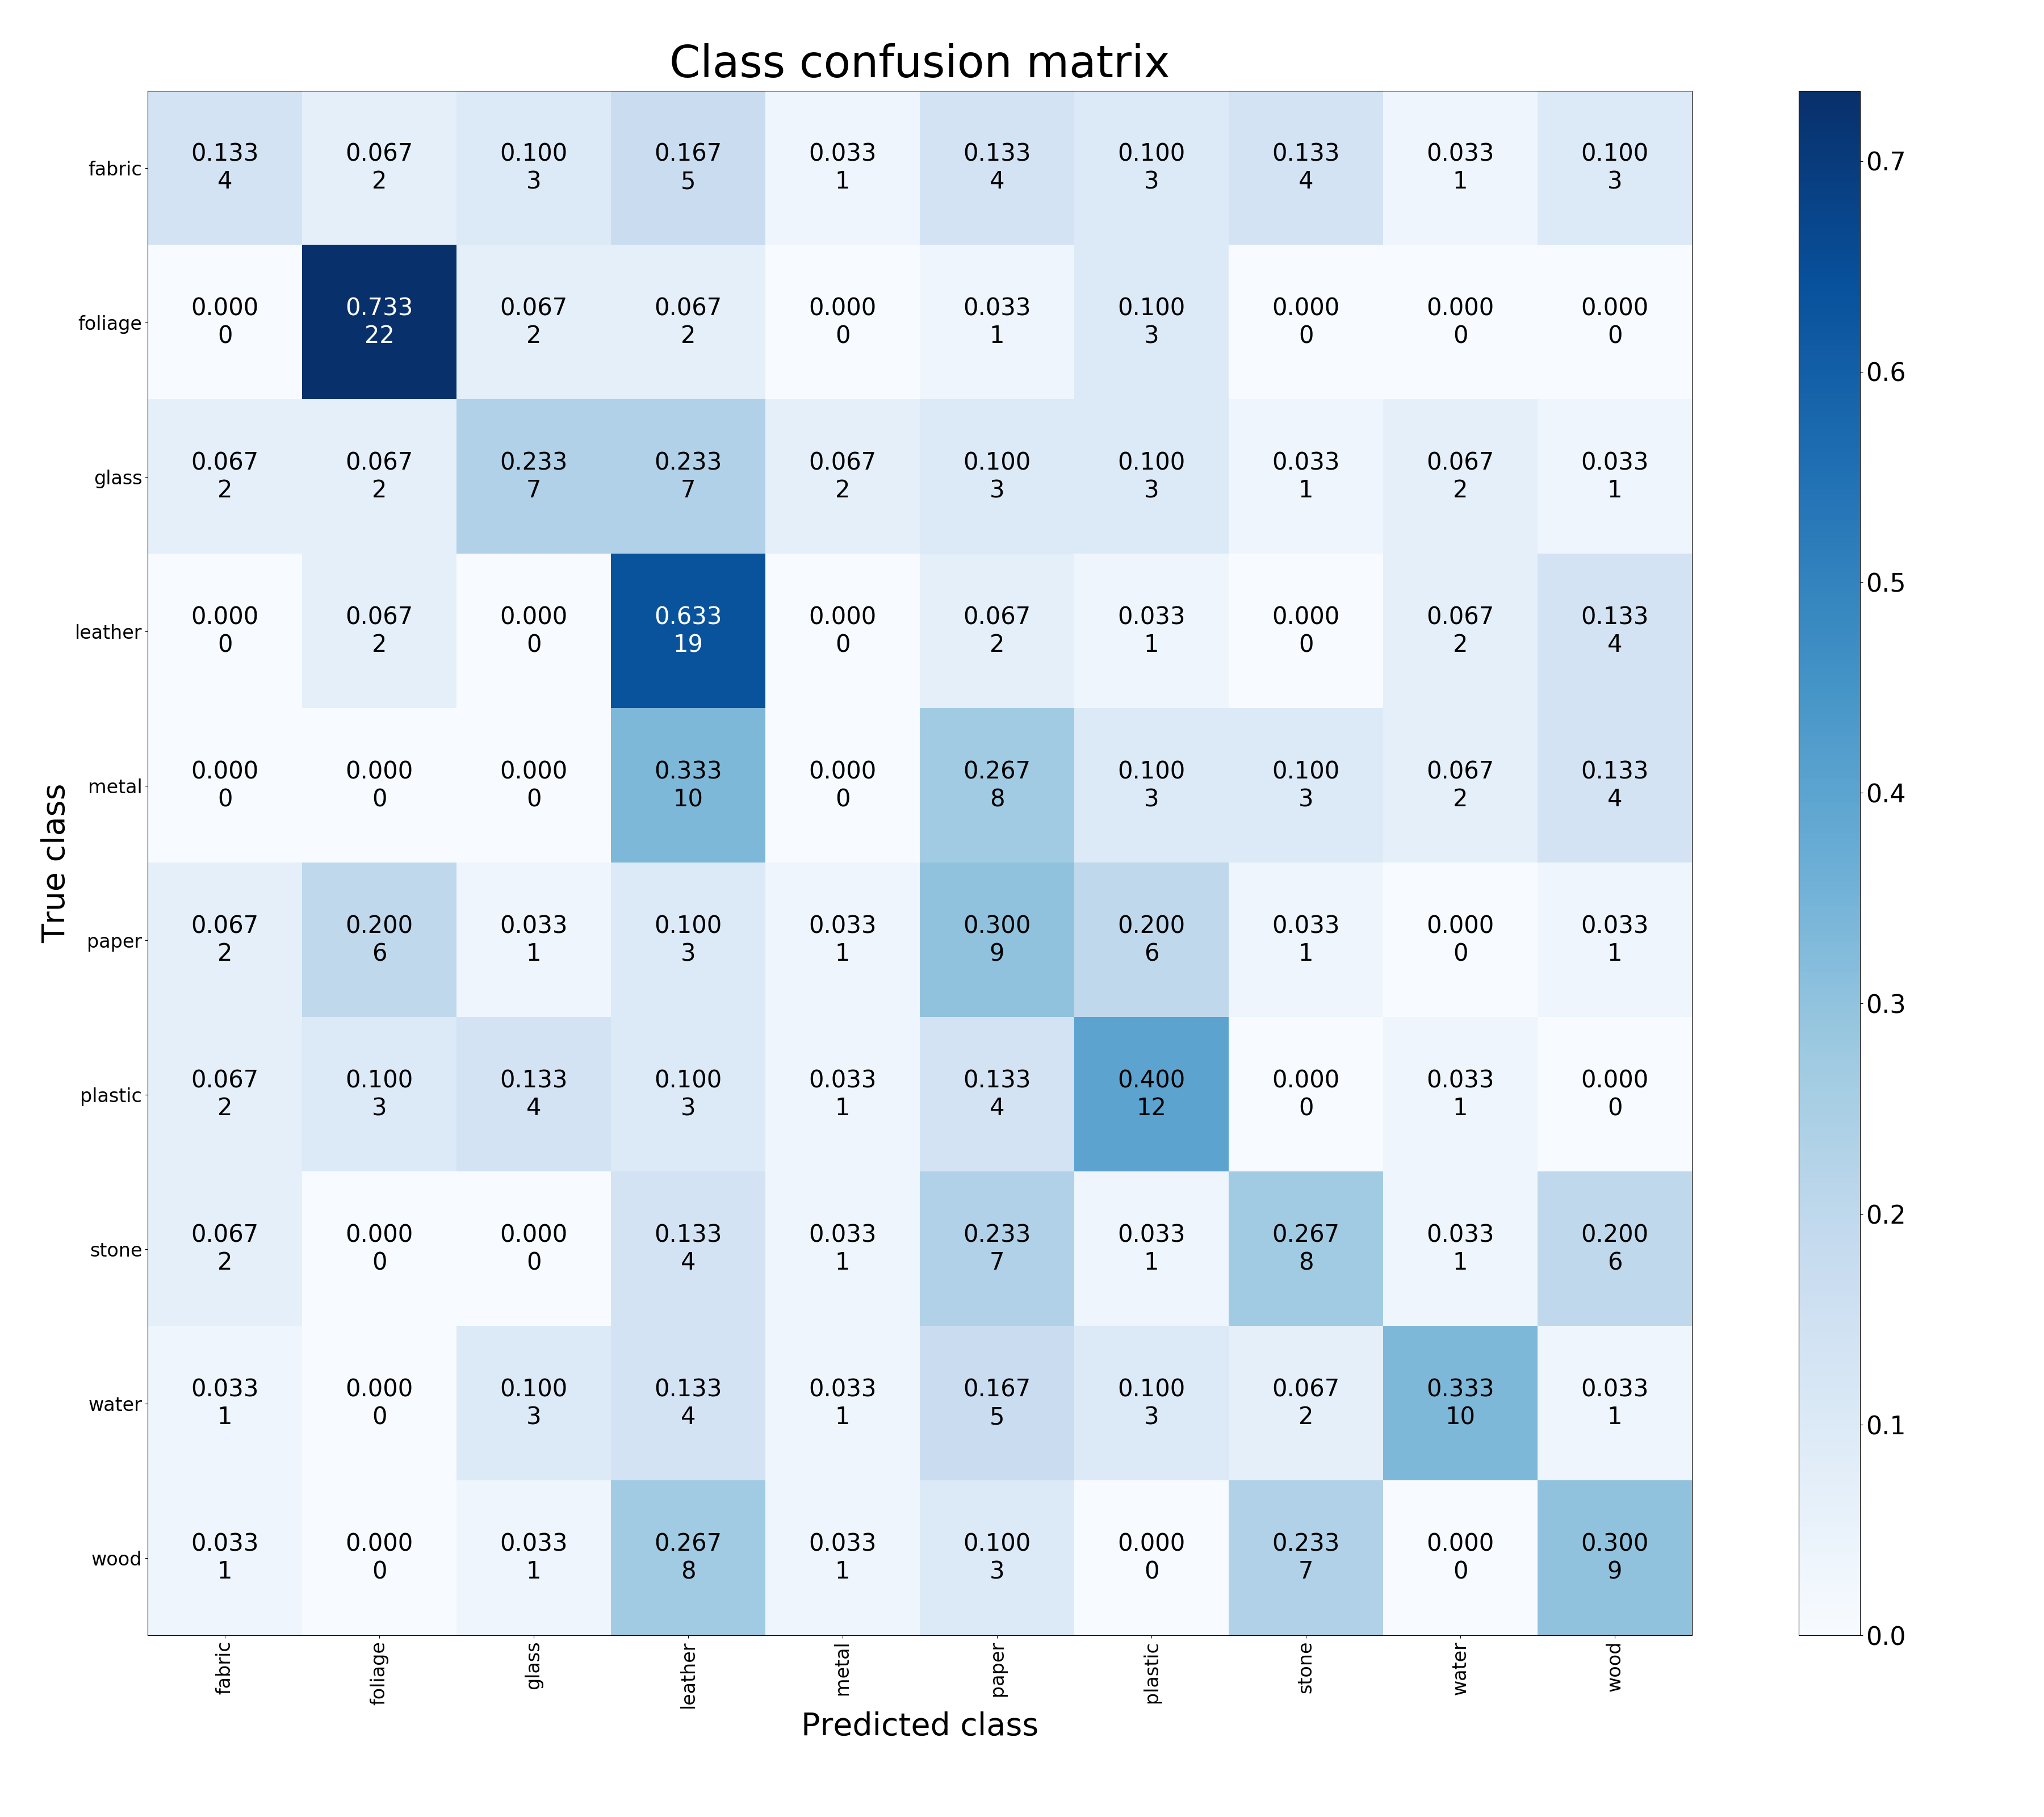
\includegraphics[width=\linewidth]{imgs/conf_fmd}
			\vspace{-7mm}
			\caption{}
			\label{fig:conffmd}
			\vspace{2mm}
		\end{subfigure}
		\caption{Confusion matrices for (a) MINC-2500 and (b) FMD predictions.}
		\label{fig:conf}
	\end{figure}

	\begin{figure}[t!]
		\centering
		\begin{subfigure}[c]{0.49\linewidth}
			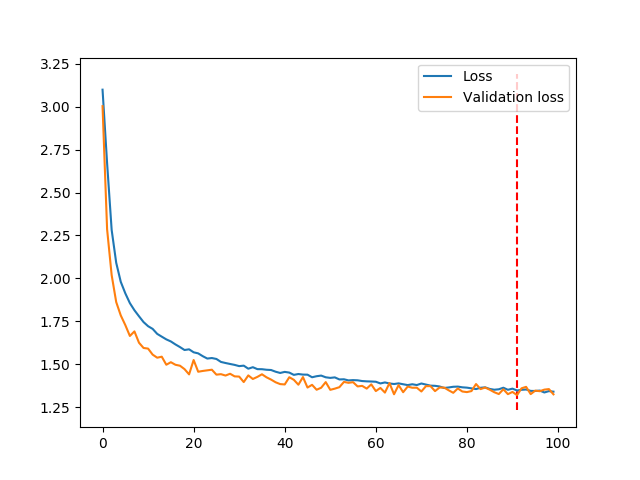
\includegraphics[width=\linewidth]{imgs/loss_history_minc}
			\caption{}
			\label{fig:lossminc}
		\end{subfigure}
		\begin{subfigure}[c]{0.49\linewidth}
			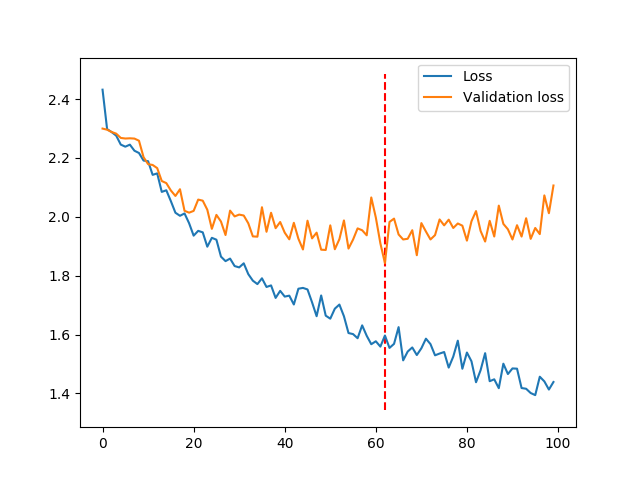
\includegraphics[width=\linewidth]{imgs/loss_history_fmd}
			\caption{}
			\label{fig:lossfmd}
		\end{subfigure}
		\caption{Training and validation losses as functions of training epochs for (a) MINC and (b) FMD datasets. The red dashed line denotes the epoch with lowest validation loss.}
		\label{fig:losses}
	\end{figure}

	\begin{table}
		\centering
		\caption{The precision and recall rates of all the categories on the MINC-2500 and FMD datasets.}
		\begin{tabular}{l|c c|c c}
			 	& \multicolumn{2}{c|}{MINC-2500}& \multicolumn{2}{c}{FMD} 	\\ \hline
			Category 		& Precision	& Recall 	& Precision	& Recall	\\ \hline
			Brick			& 0.755		& 0.644		& 			& 		\\ \hline
			Carpet			& 0.482		& 0.727		& 			& 		\\ \hline
			Ceramic			& 0.484		& 0.357		& 			& 		\\ \hline
			Fabric			& 0.401		& 0.287		& 0.286 	& 0.133	\\ \hline
			Foliage			& 0.690		& 0.811		& 0.595 	& 0.733	\\ \hline
			Food			& 0.685		& 0.799		& 			& 		\\ \hline
			Glass			& 0.582		& 0.492		& 0.333 	& 0.233	\\ \hline
			Hair			& 0.629		& 0.791		& 			& 		\\ \hline
			Leather			& 0.589		& 0.629		& 0.292 	& 0.633	\\ \hline
			Metal			& 0.340		& 0.413		& 0 		& 0		\\ \hline
			Mirror			& 0.561		& 0.487		& 			& 		\\ \hline
			Other			& 0.735		& 0.613		& 			& 		\\ \hline
			Painted			& 0.630		& 0.655		& 			& 		\\ \hline
			Paper			& 0.552		& 0.503		& 0.200 	& 0.300	\\ \hline
			Plastic			& 0.311		& 0.297		& 0.343 	& 0.400	\\ \hline
			Polished stone	& 0.645		& 0.557		& 			& 		\\ \hline
			Skin			& 0.620		& 0.673		& 			& 		\\ \hline
			Sky				& 0.923		& 0.911		& 			& 		\\ \hline
			Stone			& 0.471		& 0.613		& 0.308 	& 0.267	\\ \hline
			Tile			& 0.568		& 0.445		& 			& 		\\ \hline
			Wallpaper		& 0.663		& 0.647		& 			& 		\\ \hline
			Water			& 0.756		& 0.736		& 0.526 	& 0.333	\\ \hline
			Wood			& 0.475		& 0.425		& 0.310 	& 0.300	\\ \hline
		\end{tabular}
	\label{table:prec_rec}
	\end{table}
	
	\section{Conclusions}
	
	The deep learning models used here reached accuracies of 58.7\% and 33.3\% on the MINC-2500 and FMD datasets, respectively. This result fails to match the performance level of state-of-the-art models trained with transfer learning, which have been shown to reach over 80\% accuracy on both datasets \cite{bell_2015,zhang_2015}. The performance on the larger MINC-2500 dataset was better than on the smaller FMD dataset, even though FMD classification task should be easier in principle due to the images being more centered on the materials to be identified. In the loss curves it was seen that the FMD model clearly overfitted to the training data. This result highlights the importance of a large and varied dataset in deep learning. 
	
	\printbibliography
	
	\end{document}
